\documentclass[10pt,letterpaper]{article}
\usepackage[utf8]{inputenc}
\usepackage{graphicx}
\usepackage{caption}
\usepackage{subcaption}
\author{Michael D. Brothers}
\title{Homework 5}
\begin{document}

%{\centering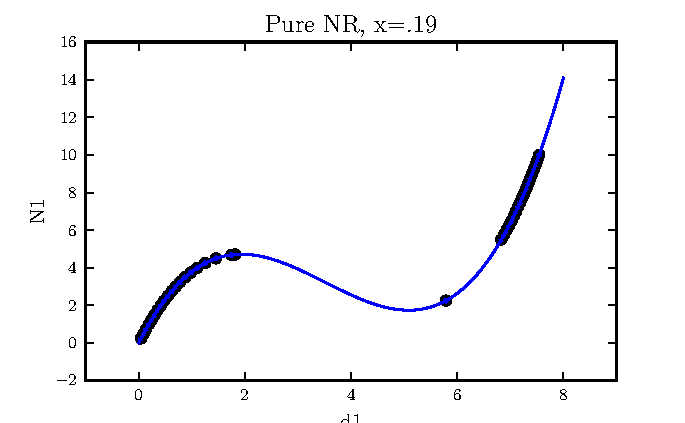
\includegraphics[width=1\textwidth]{pure_nr_x19.pdf}}
\section{Plots}

\begin{figure}[!tbh]
  \begin{subfigure}[b]{.6\textwidth}
    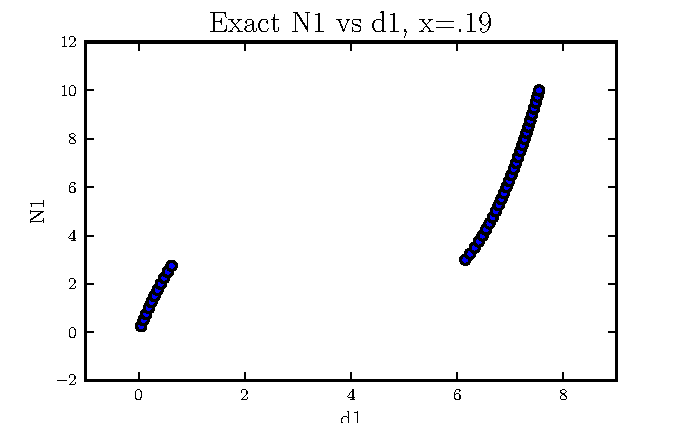
\includegraphics[width=\textwidth]{exact_x19.pdf}
    \caption{}
    \label{fig1:label:a}
  \end{subfigure}
  \hfill
  \begin{subfigure}[b]{.6\textwidth}
    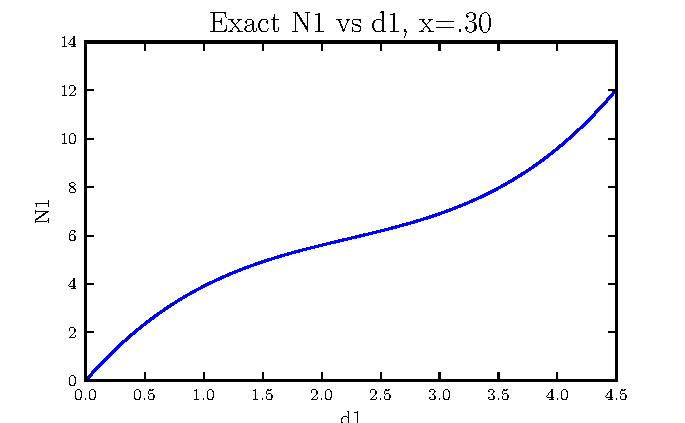
\includegraphics[width=\textwidth]{exact_x30.pdf}
    \caption{}
    \label{fig1:label:b}
  \end{subfigure}
  \caption{Exact solution curve, bisection method. There is a large jump in force values seen in~\ref{fig1:label:a}, where the true function is very flat. This jump is not seen in ~\ref{fig1:label:b}. Overall the numerical methods handled $x=.19$ worse than $x=.30$ most likely due to the flattness of the response at $x=.19$.
}
\end{figure}


\begin{figure}[!tbh]
  \begin{subfigure}[b]{.6\textwidth}
    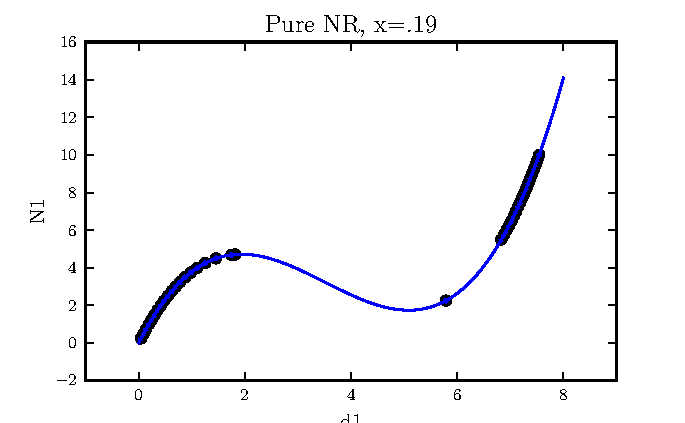
\includegraphics[width=1\textwidth]{pure_nr_x19.pdf}
    \caption{}
    \label{fig2:label:a}
  \end{subfigure}
  \hfill
  \begin{subfigure}[b]{.6\textwidth}
    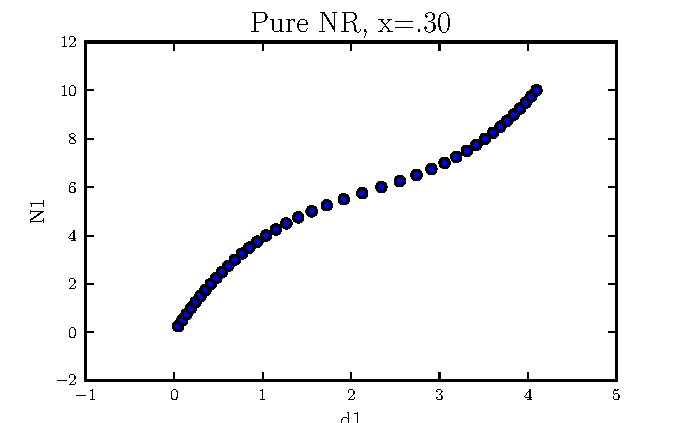
\includegraphics[width=1\textwidth]{pure_nr_x30.pdf}
    \caption{}
    \label{fig2:label:b}
  \end{subfigure}
  \hfill
    \begin{subfigure}[b]{.6\textwidth}
    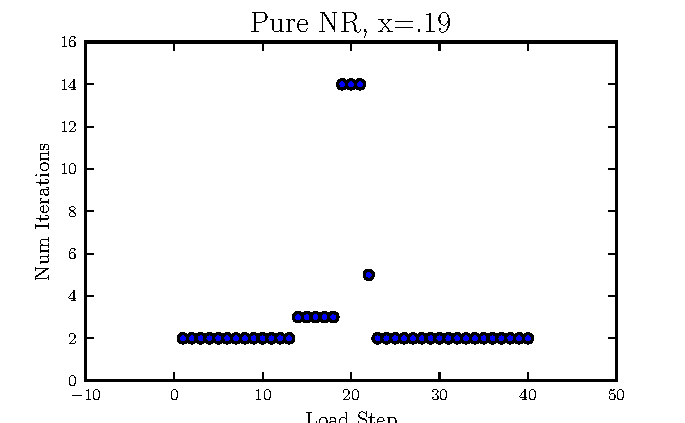
\includegraphics[width=1\textwidth]{pure_nr_x19_conv.pdf}
    \caption{}
    \label{fig2:label:c}
  \end{subfigure}
  \hfill
  \begin{subfigure}[b]{.6\textwidth}
    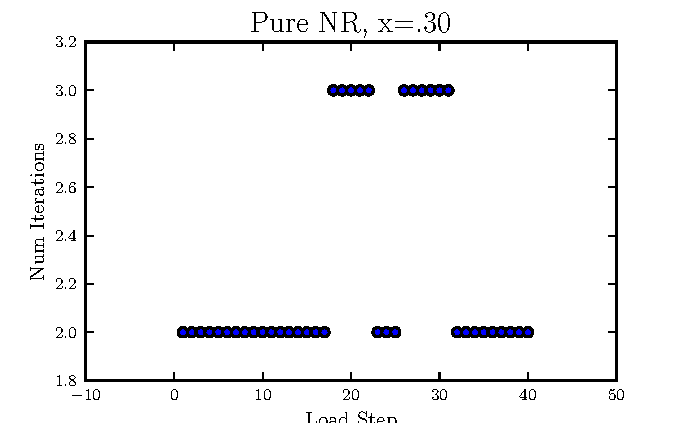
\includegraphics[width=1\textwidth]{pure_nr_x30_conv.pdf}
    \caption{}
    \label{fig2:label:d}
  \end{subfigure}
  \caption{Numerical solution curve, NR method. Looking at~\ref{fig2:label:c} the pure Newton Raphson method failed to converge after $18$ loadsteps in that case that $x=.19$. The method converged to approximate solutions for all loadsteps for the case that $x=.30$.
}
\end{figure}


\begin{figure}[!tbh]
  \begin{subfigure}[b]{.6\textwidth}
    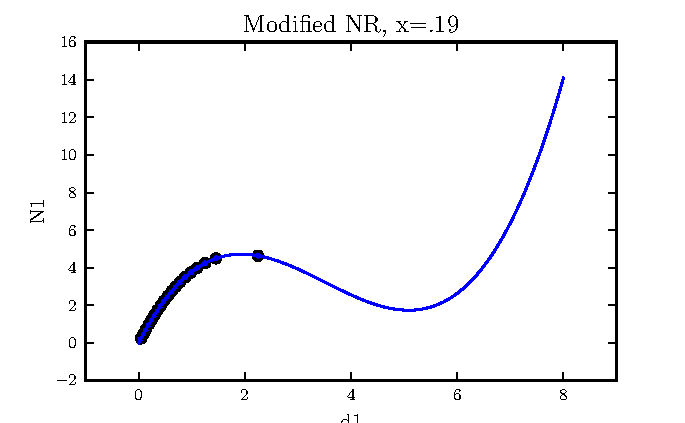
\includegraphics[width=\textwidth]{moded_nr_x19.pdf}
    \caption{}
    \label{fig3:label:a}
  \end{subfigure}
  \hfill
  \begin{subfigure}[b]{.6\textwidth}
    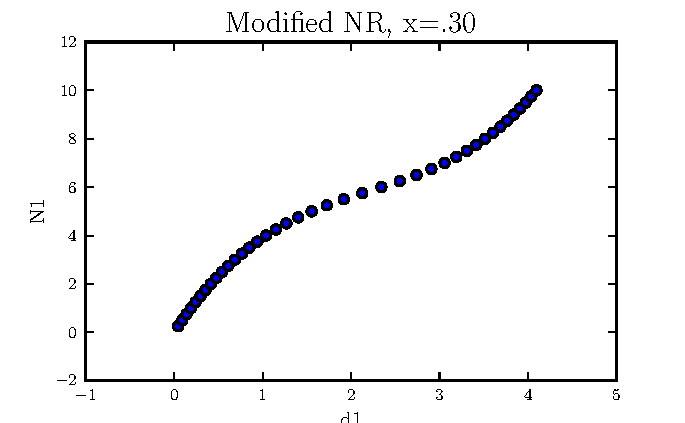
\includegraphics[width=\textwidth]{moded_nr_x30.pdf}
    \caption{}
    \label{fig3:label:b}
  \end{subfigure}
  \hfill
    \begin{subfigure}[b]{.6\textwidth}
    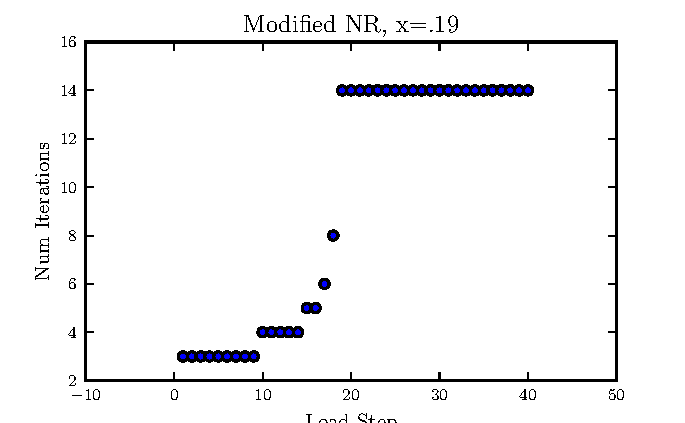
\includegraphics[width=\textwidth]{moded_nr_x19_conv.pdf}
    \caption{}
    \label{fig3:label:c}
  \end{subfigure}
  \hfill
  \begin{subfigure}[b]{.6\textwidth}
    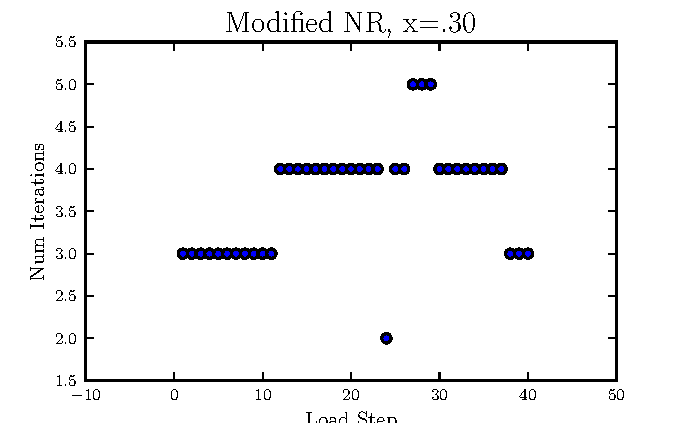
\includegraphics[width=\textwidth]{moded_nr_x30_conv.pdf}
    \caption{}
    \label{fig3:label:d}
  \end{subfigure}
  \caption{Numerical solution curve, modified NR method. Looking at~\ref{fig3:label:c} the modified Newton Raphson method failed to converge after $18$ loadsteps in that case that $x=.19$. The method converged to approximate solutions for all loadsteps for the case that $x=.30$.
 }
\end{figure}

\begin{figure}[!tbh]
  \begin{subfigure}[b]{.6\textwidth}
    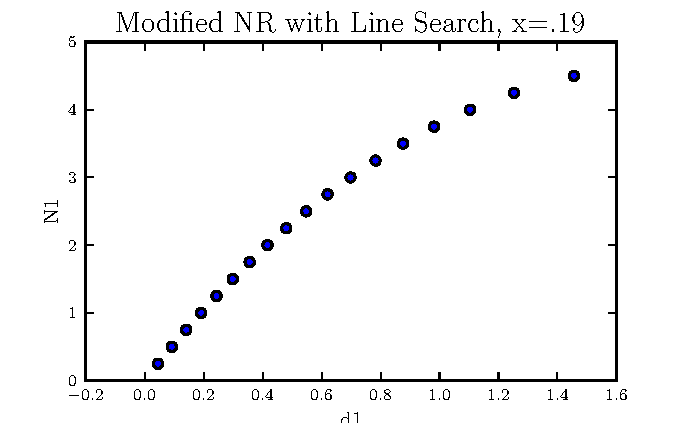
\includegraphics[width=\textwidth]{moded_nr_wls_x19.pdf}
    \caption{}
    \label{fig4:label:a}
  \end{subfigure}
  \hfill
  \begin{subfigure}[b]{.6\textwidth}
    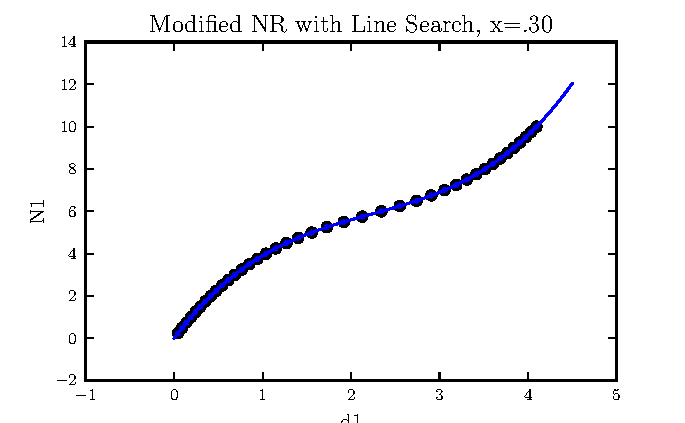
\includegraphics[width=\textwidth]{moded_nr_wls_x30.pdf}
    \caption{}
    \label{fig4:label:b}
  \end{subfigure}
  \hfill
    \begin{subfigure}[b]{.6\textwidth}
    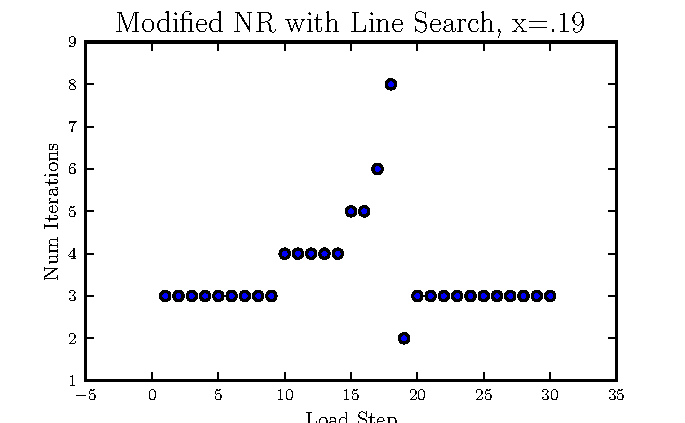
\includegraphics[width=\textwidth]{moded_nr_wls_x19_conv.pdf}
    \caption{}
    \label{fig4:label:c}
  \end{subfigure}
  \hfill
  \begin{subfigure}[b]{.6\textwidth}
    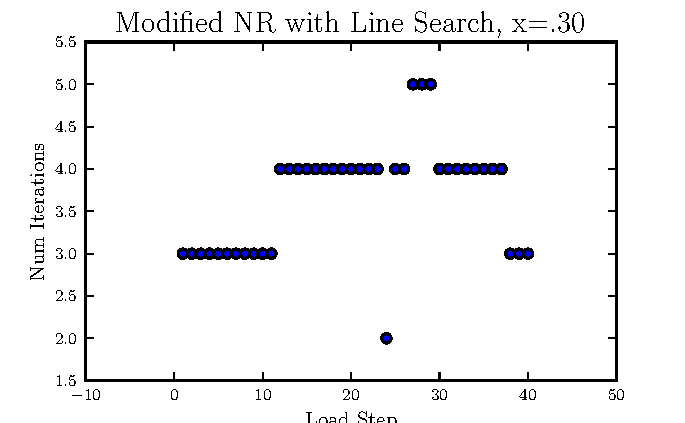
\includegraphics[width=\textwidth]{moded_nr_wls_x30_conv.pdf}
    \caption{}
    \label{fig4:label:d}
  \end{subfigure}
    \caption{Numerical solution curve, modified NR method with line search. Looking at~\ref{fig4:label:c} the modified Newton Raphson method with line search failed to converge after $18$ loadsteps in that case that $x=.19$. The method converged to approximate solutions for all loadsteps for the case that $x=.30$.
 }
\end{figure}

\begin{figure}[!tbh]
  \begin{subfigure}[b]{.6\textwidth}
    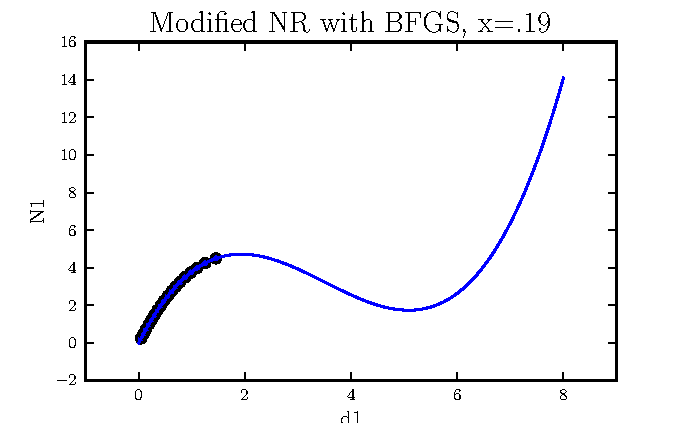
\includegraphics[width=\textwidth]{moded_nr_bfgs_x19.pdf}
    \caption{}
    \label{fig5:label:a}
  \end{subfigure}
  \hfill
  \begin{subfigure}[b]{.6\textwidth}
    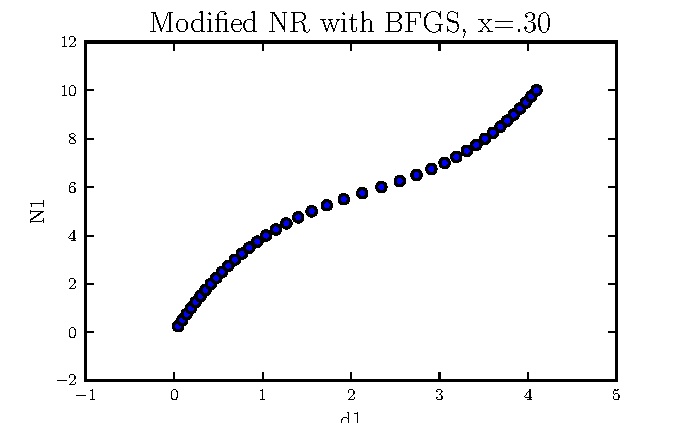
\includegraphics[width=\textwidth]{moded_nr_bfgs_x30.pdf}
    \caption{}
    \label{fig5:label:b}
  \end{subfigure}
  \hfill
    \begin{subfigure}[b]{.6\textwidth}
    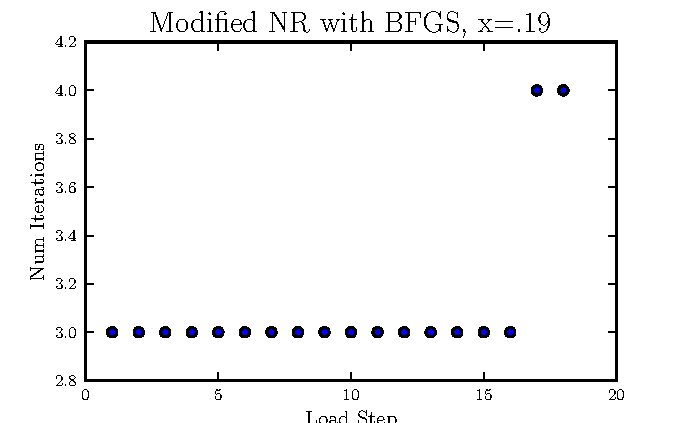
\includegraphics[width=\textwidth]{moded_nr_bfgs_x19_conv.pdf}
    \caption{}
    \label{fig5:label:c}
  \end{subfigure}
  \hfill
  \begin{subfigure}[b]{.6\textwidth}
    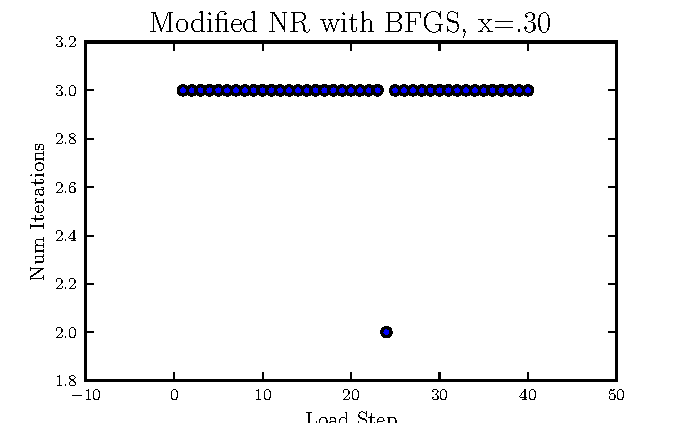
\includegraphics[width=\textwidth]{moded_nr_bfgs_x30_conv.pdf}
    \caption{}
    \label{fig5:label:d}
  \end{subfigure}
    \caption{Numerical solution curve, modified NR method with BFGS. Looking at~\ref{fig5:label:c} the modified Newton Raphson method with BFGS failed to converge after $18$ loadsteps in that case that $x=.19$. The method converged to approximate solutions for all loadsteps for the case that $x=.30$.
 }
\end{figure}

\begin{figure}[!tbh]
  \begin{subfigure}[b]{.6\textwidth}
    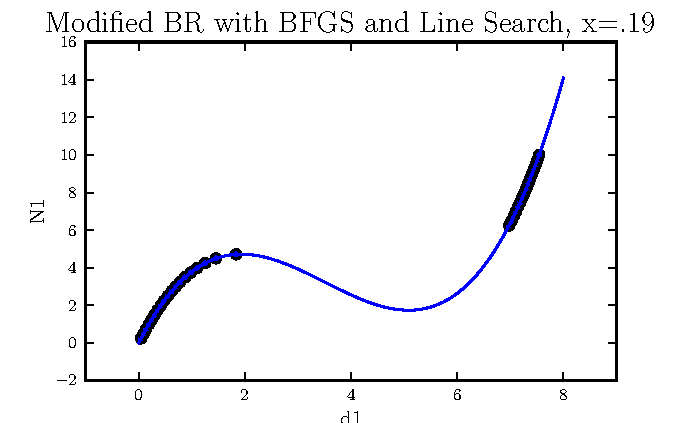
\includegraphics[width=\textwidth]{moded_nr_bfgs_wls_x19.pdf}
    \caption{}
    \label{fig6:label:a}
  \end{subfigure}
  \hfill
  \begin{subfigure}[b]{.6\textwidth}
    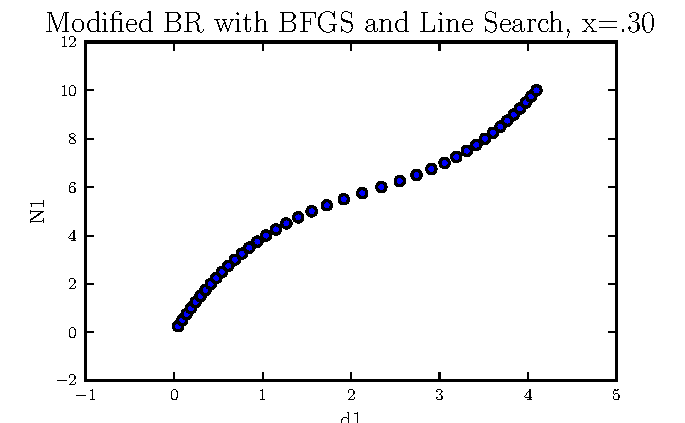
\includegraphics[width=\textwidth]{moded_nr_bfgs_wls_x30.pdf}
    \caption{}
    \label{fig6:label:b}
  \end{subfigure}
  \hfill
    \begin{subfigure}[b]{.6\textwidth}
    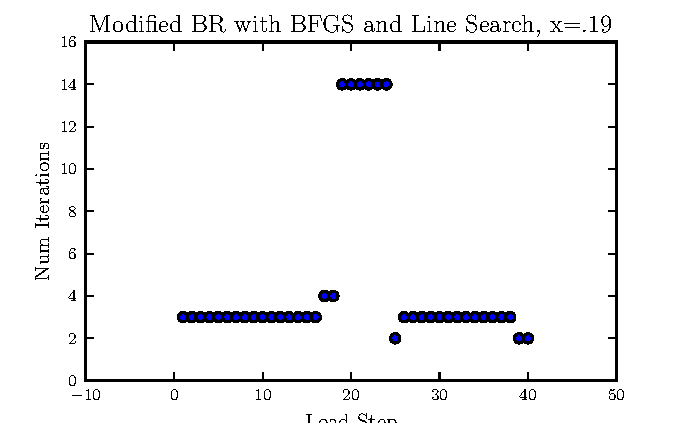
\includegraphics[width=\textwidth]{moded_nr_bfgs_wls_x19_conv.pdf}
    \caption{}
    \label{fig6:label:c}
  \end{subfigure}
  \hfill
  \begin{subfigure}[b]{.6\textwidth}
    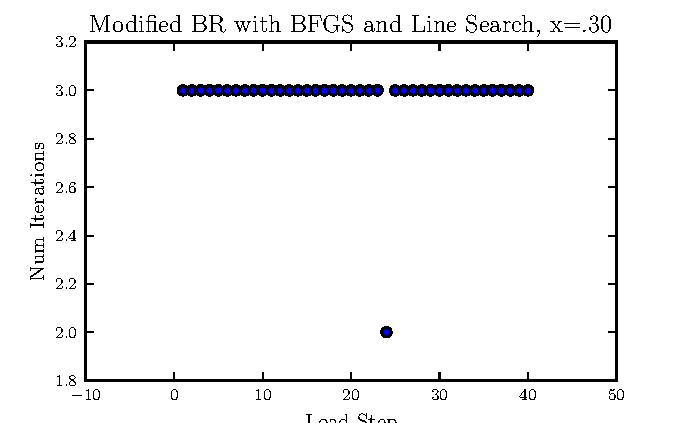
\includegraphics[width=\textwidth]{moded_nr_bfgs_wls_x30_conv.pdf}
    \caption{}
    \label{fig6:label:d}
  \end{subfigure}
    \caption{Numerical solution curve, modified NR method with BFGS and line search. Looking at~\ref{fig6:label:c} the modified Newton Raphson method with BFGS and line search failed to converge after $18$ loadsteps in that case that $x=.19$. The method converged to approximate solutions for all loadsteps for the case that $x=.30$.
 }
\end{figure}

\end{document}
